
\section*{Problema P7.29}

\renewcommand*\thesection{7.29}
\numberwithin{equation}{section}

\begin{center}
    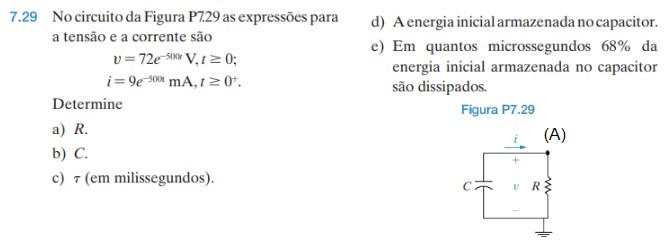
\includegraphics[scale=1.0]{P7.29.jpg}
\end{center}

Antes de tudo, vamos extrair a função de $v(t)$ genérica para o circuito. 
Aplicamos análise nodal no nó (A) da figura, obtendo    

\[ -i + \frac{V_A}{R} = 0 \]

Em um capacitor, sabemos que 

\begin{equation}\label{eq:7.29.1}
    i(t) = C\diff{v}{t}
\end{equation}

Note que $i$ está entrando no terminal negativo de $C$. Assim, usamos sinal negativo em \eqref{eq:7.29.1} para manter a 
convenção passiva. Substituindo \eqref{eq:7.29.1} na equação nodal, e usando $v = V_A$, temos   

\[ -\left(-C\diff{v}{t}\right) + \frac{v}{R} = 0 \]

\[ \diff{v}{t} + \frac{v}{RC} = 0 \]

Usando o fator integrante $M(t) = e^{\frac{1}{RC}t}$, temos   

\[ e^{-\frac{1}{RC}t}\diff{v}{t} + e^{\frac{1}{RC}t}\frac{v}{RC} = 0 \]

Aplicando o inverso da regra da derivada do produto,

\[ \diff{[v(t) \cdot e^{\frac{1}{RC}t}]}{t} = 0 \]

\[ v(t) \cdot e^{\frac{1}{RC}t} = K \]

\begin{equation}\label{eq:7.29.2}
    v(t) = Ke^{-\frac{1}{RC}t} \un{V} \, , \, t \geq 0
\end{equation}

\subsection*{(a)}

Usando a Lei de Ohm,  

\[ \boxed{R = \frac{v(t)}{i(t)} = \frac{72e^{-500t} \un{V}}{9e^{-500t} \un{mA}} = 8\un{k$\Omega$}}  \]

\subsection*{(b)}

Comparando \eqref{eq:7.29.1} com a função de $v(t)$ dada no exercício, temos   

\[ -\frac{1}{RC} = -500 \]

\[ C = -\frac{1}{R(-500)} \]

\[ \boxed{C = 250 \un{nF}}  \]

\subsection*{(c)}

A constante de tempo $\tau$ é definida como

\begin{equation}\label{eq:7.29.3}
    \tau = RC
\end{equation}

Assim,

\[ \boxed{\tau = 2 \un{ms}}  \]

\subsection*{(d)}

A energia no capacitor é dada por   

\begin{equation}\label{eq:7.29.4}
    E(t) = \frac{1}{2}C[v(t)]^2
\end{equation}

Assim, em $t=0$, temos a energia inicial  

\[ E(0) = \frac{1}{2}(250 \un{nF})[72\un{V}]^2  \]

\[ \boxed{E(0) = 648 \un{$\mu$J}}  \]

\subsection*{(e)}

Isolando $t$ em \eqref{eq:7.29.4}, 

\[ v(t) = \sqrt{\frac{2E(t)}{C}}  \]

Substituindo a função de $v(t)$ do enunciado na expressão acima, temos   

\[ e^{-\frac{t}{RC}} = \frac{1}{v_0} \sqrt{\frac{2E(t)}{C}}  \]

\[ -\frac{t}{RC} = \ln \left(\frac{1}{v_0} \sqrt{\frac{2E(t)}{C}}\right)   \]

\[ t = -RC\ln \left(\frac{1}{v_0} \sqrt{\frac{2E(t)}{C}}\right)   \]

Queremos que seja dissipado $68\%$ da energia inicial armazenada. Isso significa que precisamos de um instante $t$ tal que

\[ E(t) = 32\% E(0) = \frac{32}{100}E(0) = \frac{32}{100}\frac{1}{2}Cv_o^2 \]

Substituindo esse $E(t)$ na expressão de $t$ acima,   

\[ t = -RC\ln \left(\frac{1}{v_0} \sqrt{\frac{2\frac{32}{100}\frac{1}{2}Cv_o^2}{C}}\right)  \]

\[ t = -RC\ln \left(\sqrt{\frac{32}{100}}\right)  \]

Substituindo tudo,   

\[ \boxed{t = 1139.43 \un{$\mu$s}}  \]















